\section{Interpreter Manipulation Method Examples}
\label{sec:manipulations}

After introducing the terminology of model interpreters and manipulation methods in the previous chapters, this chapter gives detailed information about recent manipulation methods. This section also provides insight into major findings in the field of manipulating model interpretations. First, input level manipulations are discussed, followed by model level manipulations. 

\subsection{Input Level Manipulations}

\mypar{Fooling both Model and Interpreter. }\newline
\cite{subramanya2019fooling} design adversarial attacks that fool the machine learning model as well as the model interpretation. 
They design targeted and untargeted input patches superimposed onto original images and then fed into an image classification network and the intperpretation method GradCAM. 

The authors conclude that GradCAM does not reliably highlight the true cause of the prediction decision made by the model. 
Top-1 predicted label 

The authors compare targeted and untargeted patches as well as uniform patches and randomly disturbed ones. 



\mypar{Model-agnostic Interpreters can be gamed.}\newline
%%%%%%%%  %%%%%%%% Fooling LIME and SHAP: Adversarial Attacks on Post hoc Explanation Methods
% https://arxiv.org/pdf/1911.02508.pdf 
\cite{advlime_aies20} propose a framework for fooling the model-agnostic interpreters LIME and SHAP. Their method successfully hides the biases of models trained on adversarial examples by... 
The authors take a statistical approach model-agnostic interpretation methods. They examined the data produced by LIME and SHAP and showed that the perturbed samples are out-of-distrubution samples compared to the distribution of the regular trainging data. 

\autoref{fig:slack_ood_data} shows that the data samples generated by LIME are distributed differently than the data original, non-perturbed data samples. 

\begin{figure}[ht]
    \centering
    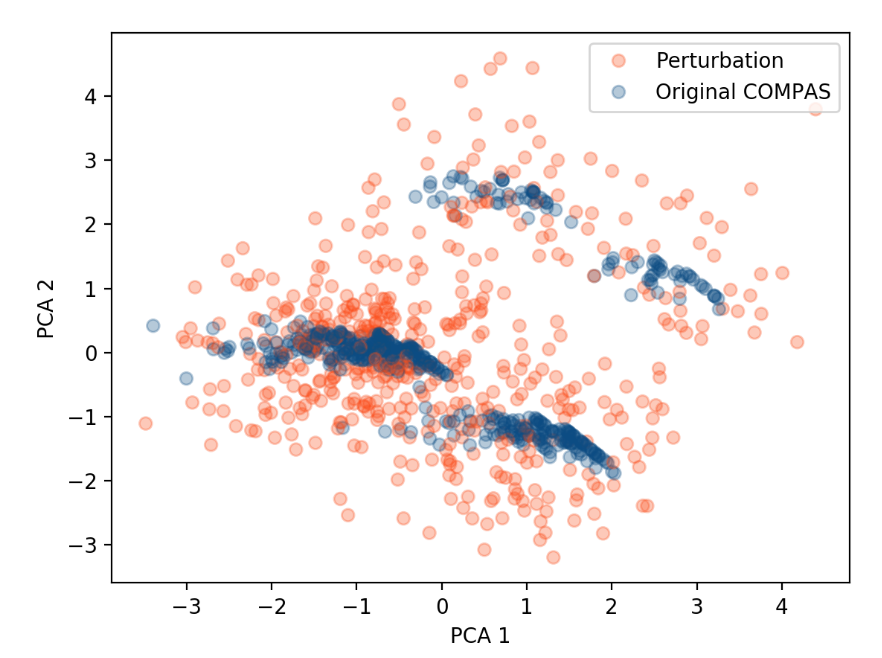
\includegraphics[width=\linewidth]{figures/slack_ood_data.png}
    \caption{Principal Component Analysis (PCA) on the original data (orange) of the COMPAS dataset and the samples perturbed by LIME (blue). Note that the differences are obvious even in the space reduced to two dimensions.}
    \label{fig:slack_ood_data}
    \vspace{-0.3cm}
\end{figure}

\mypar{Saliency Maps are vulnerable to Adversarial Attacks.}
\cite{ghorbani2019interpretation} showed that importance scores produced by the popular interpretation methods Simple Grad, DeepLIFT and TODO. 



\subsection{Model Level Manipulations}

\mypar{Adversarial Model Manipulations can fool a wide range of interpreters.}
\cite{fooling_nn_interpreters} were the first to introduce adversarial model manipulations for fooling interpretation methods. 
Their research question is if state-of-the-art interpretation methods be fooled with adversarial model manipulations. For this, the authors adapted the fine-tuning of image-classification models by using an altered loss function. 
After fine-tuning the model with the regular classification loss combined with an adversarial loss, they investigated if the interpreter results change as a function of model parameters. 
Two types of fooling methods were introduced, namely \textit{active} and \textit{passive} fooling. 

% HEO: The authors find that perturbed model parameters can also make explanations worse for the same input images and interpreters. 
% \subsubsection{Transferability of Manipulations}
% \cite{fooling_nn_interpreters} find that fooling one explanation method with a fooling scheme transfers to other methods. 

%%%%%%%%  %%%%%%%%
\mypar{}
\cite{dimanov2020you} examine the relation of interpretation methods and the concept of fairness. They propose to learn a modified model with concealed unfairness. This is done by fine-tuning a classification model with a loss function extended by an explanation loss. 

Their approach differs methodologically to \cite{fooling_nn_interpreters} as follows: 
\cite{fooling_nn_interpreters} adapt the standard cross entropy loss function by taking the gradient of the correct label ellement from the logits layer, while \cite{dimanov2020you} use the gradient of the cross-entopy loss. 
Taking the gradient of the cross-entropy loss conveys more information about other classes, which may contribute to an improved generalization across different interpretation methods and first of all across different test samples. 

While their approach takes the gradient of the onecorrect label element from the logits layer just before thesoftmax output, we take the gradient of the cross-entropyloss. 

They define adversarial models that focus only on sensitive features which are not informative for the ground truth decision. 


%%%%%%%%%%%%%%
% Conclusions based on the presented studies
